% Gemini theme
% https://github.com/anishathalye/gemini

\documentclass[final]{beamer}

% ====================
% Packages
% ====================

\usepackage[T1]{fontenc}
\usepackage{lmodern}
\usepackage[size=custom,width=48,height=36,scale=0.4]{beamerposter}
\usetheme{gemini}
\usecolortheme{gemini}
\usepackage{graphicx}
\usepackage{booktabs}
\usepackage{tikz}
\usepackage{pgfplots}
\pgfplotsset{compat=1.14}
\usepackage{anyfontsize}
\usepackage{amsmath}
\usepackage{wrapfig}

% ====================
% Lengths
% ====================

% If you have N columns, choose \sepwidth and \colwidth such that
% (N+1)*\sepwidth + N*\colwidth = \paperwidth
\newlength{\sepwidth}
\newlength{\colwidth}
\setlength{\sepwidth}{0.025\paperwidth}
\setlength{\colwidth}{0.3\paperwidth}

\newcommand{\separatorcolumn}{\begin{column}{\sepwidth}\end{column}}

% ====================
% Title
% ====================

\title{\centering Causal Discovery on Gut Microbial Data for Disease Risk Prediction}

\author{Mariana Paco Mendivil \inst{1} \and Candus Shi \inst{2} \and Nicole Zhang \inst{3} \and Mentor: Biwei Huang \inst{4} \and Mentor: Jelena Bradic \inst{5}}
 
\institute[shortinst]{\inst{1} mpacomendivil@ucsd.edu \samelineand \inst{2} c6shi@ucsd.edu \samelineand \inst{3} nwzhang@ucsd.edu \samelineand \inst{4} bih007@ucsd.edu \samelineand \inst{5} jbradic@ucsd.edu}

% \author{\vspace{1cm} \hspace{1cm} \raggedright Mariana Paco Mendivil \and Candus Shi \and Nicole Zhang }

% \institute {\hspace{1.6cm} \raggedright mpacomendivil@ucsd.edu \samelineand \hspace{1.2cm} c6shi@ucsd.edu \hspace{1cm} nwzhang@ucsd.edu}

% ====================
% Footer (optional)
% ====================

\footercontent{
  Please visit our website at \href{https://nzhang20.github.io/Causal-Discovery-on-Gut-Microbial-Data-for-Disease-Risk-Prediction/}{https://nzhang20.github.io/Causal-Discovery-on-Gut-Microbial-Data-for-Disease-Risk-Prediction/} or at the above QR code.}
% (can be left out to remove footer)

% ====================
% Logo (optional)
% ====================

% use this to include logos on the left and/or right side of the header:
\logoright{\includegraphics[height=1.5cm]{hdsi-white.png}}
% \logoleft{\includegraphics[height=7cm]{logo2.pdf}}

% ====================
% Body
% ====================

\begin{document}

\begin{frame}[t]
\begin{columns}[t]
\separatorcolumn

\begin{column}{\colwidth}

  \begin{block}{Background}
    \begin{itemize}
      \item \textbf{Causal Discovery \& Causal Inference:} These are a set of methods and models that attempt to causally answer scientific questions using observed data rather than RCTs.
      \item \textbf{Gut Microbiome:} The gut microbiome is an important indicator of human health, and extensive research is ongoing to explore its impact on human health and disease.
      \item \textbf{Causality in the Gut Microbiome:} Most studies report associations, but these are often insufficient to answer the scientific question of interest.
      % \item \textbf{Causal Discovery and Inference in the Gut Microbiome:} Previous work has attempted causal discovery in gut microbiome studies, using PC-stable to construct causal networks and implement do-calculus for estimating microbe-microbe and microbe-outcome causal effects. 
    \end{itemize}

  \end{block}
  
  \vspace{0.5cm}

  \begin{block}{Research Questions}

    \begin{enumerate}
      \item \textbf{Microbe-Microbe:} How do the microbe-microbe interaction networks between healthy and diseased participants differ?
      \item \textbf{Microbe-Disease:} Which microbes have a causal relationship to disease status, and how is it quantified?
      \item \textbf{Prediction:} Is it possible to predict disease status with the current composition of the dataset given causal representation learning techniques? How do they differ with the microbes learned in question 2?
    \end{enumerate}
  \end{block}
  
  \vspace{0.5cm}

  \begin{block}{Data}

   % We apply our framework to gut microbial data that studied T2D and PCOS. 
    
    \begin{itemize}
      \item \textbf{T2D:} NIH Human Microbiome Project (HMP2) dataset, filtered to healthy visits with 16S sequencing. Includes 153 insulin-sensitive (IS) and 178 insulin-resistant (IR) samples.
      \item \textbf{PCOS:} Meta analysis dataset from 14 different clinical studies across Asia and Europe. Includes 435 healthy controls (HC) and 513 PCOS patients.
    \end{itemize}

  \end{block}
  
  \vspace{0.5cm}
  
	  \begin{alertblock}{Causal Discovery}
	  
	  	Causal discovery attempts to recover the true causal structure of a system given observed data. One way to model this causal structure is through a directed graphical model. A widely-used general-purpose causal discovery algorithm is the Peter-Clark (PC) algorithm. It follows these key steps:
		\begin{enumerate}
		    \item Start with a \textbf{complete undirected graph} (each node connected to all other nodes).
		    \item \textbf{Remove edges} based on statistical independence and conditional independence tests.
		    \item \textbf{Identify v-structures} (patterns like $X \to Y \leftarrow Z$) to infer causal directions.
		    \item \textbf{Apply Meek’s rules} to orient additional edges while preserving v-structures.
		\end{enumerate}

	The result is a \textbf{CPDAG (Completed Partially Directed Acyclic Graph)}, which represents a set of causal structures consistent with the observed data, also known as the Markov Equivalence Class (MEC). 

%	\textbf{\underline{Why Use PC?}}
%			\begin{itemize}
%			    \item Works for different data types (as long as independence tests match the data distribution).
%			    \item Efficient for large datasets.
%			    \item Assumes the \textbf{causal Markov condition}, the \textbf{faithfulness} assumption, and \textbf{no hidden confounders}.
%			\end{itemize}
	  
	  \end{alertblock}
	  
	  \vspace{0.5cm}
	  
\begin{block}{Methods}

%   In this study, we use causal discovery algorithms and compare them with 
%   predictive modeling to explore the causal relationships between the 
%   gut microbiome and two diseases: T2D and PCOS. Due to the high-dimensionality
%   of the data and small sample sizes, we first select features through sparse
%   estimation methods and sure-screening to reduce the number of microbes. 

    \begin{enumerate}
      \item \textbf{Filter out rare OTUs}. 
      \item \textbf{Feature selection and sure screening}. SparCC and graphical lasso to reduce the number of edges between pairs of microbes; logistic lasso regression to reduce the number of features that are not helpful in predicting disease. 
      \item \textbf{Causal discovery algorithms}. PC-stable with a max depth of 2 for microbe-microbe; CD-NOD (a variant of PC) for microbe-outcome.
      \item \textbf{Causal inference}. do-calculus and logistic regression for causal effects; compare with Bayesian Inferential Regression for Differential Microbiome Analysis (BIRDMAn).
      \item \textbf{Variational autoencoder}. xxx. Formulas.
    \end{enumerate}

  \end{block}


\end{column}

\separatorcolumn

\begin{column}{\colwidth}

  
  \begin{block}{T2D}

%    From the microbe-disease network (Figure 1), the following five genera are causal to T2D (`IRIS' node): \textit{Butyricimonas, Clostridium XIVb, Odoribacter, unclassified Bacteria,} and \textit{unclassified Firmicutes}. To further investigate their individual effects, we implement do-calculus through logistic regression models on T2D given the neighbors of the genus of interest (Table 1). We implement three models: a simple logistic regression model regressed on the five genera causal to T2D, a logistic regression model regressed on a microbe and its neighbors, and a logistic regression model regressed on a microbe and its mediators. We compare the values with the BIRDMAn's mean CLR. Their significance is denoted with an asterisk (*). 

    \begin{figure}
      \centering
      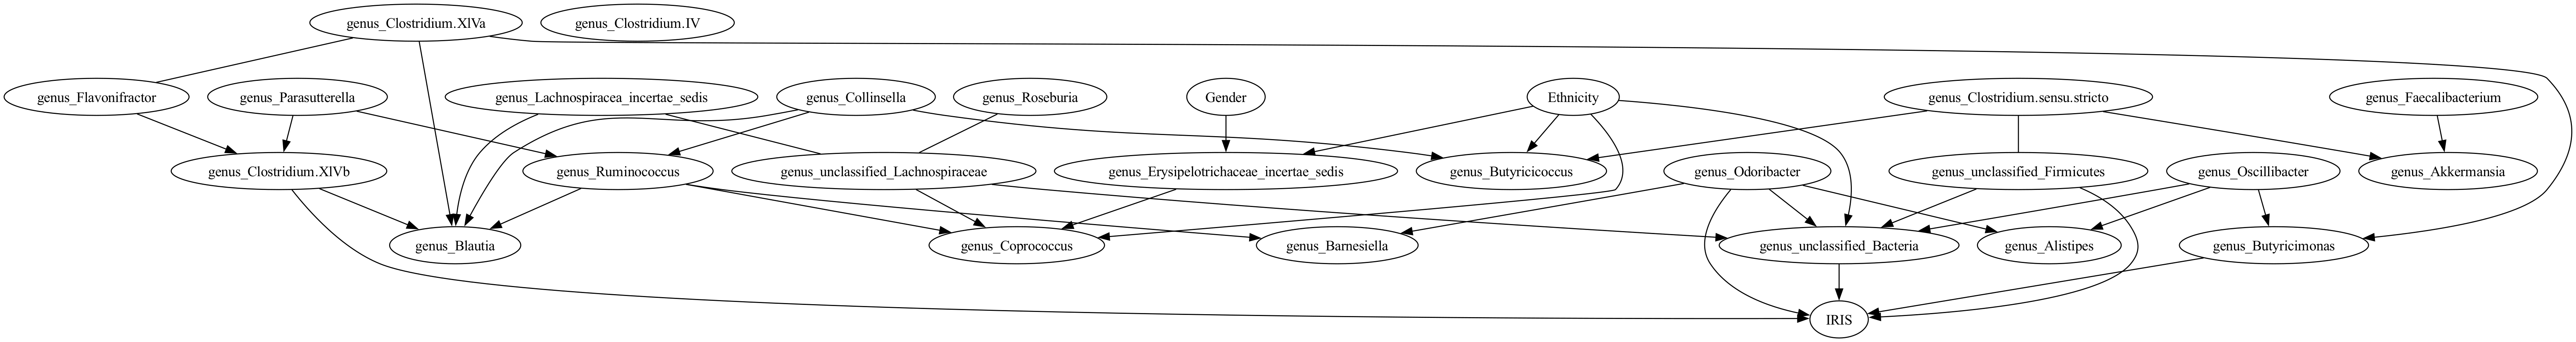
\includegraphics[width=\linewidth]{../graphs/t2d/cdnod_norm.png}
      \caption{Microbe-Disease Network for T2D.}
    \end{figure}
    
    \vspace{0.5cm}
    
    \textbf{Model 1}: logit(disease status) $\sim$ microbes directly linked \\
    \textbf{Model 2}: logit(disease status) $\sim$ microbe + neighbors(microbe) or mediators \\
    \textbf{BIRDMAn}: Bayesian inference with $NegBinomial(\mu, \phi)$ where $\mu$ is the mean count and $\phi$ is the dispersion
    
    \begin{table}
      \centering
      \begin{tabular}{l r r r c}
        \toprule
        \textbf{Genus} & \textbf{Model 1} & \textbf{Model 2} & \textbf{BIRDMAn} & \textbf{Literature Agreement} \\
        \midrule
        \textit{Butyricimonas} & -2.0070* & -2.26645* & -5.19385* & Yes \\
        \textit{Clostridium XIVb} & 1.54212* & 1.80822* & 2.15788* & Inconclusive \\
        \textit{Odoribacter} & -1.46989* & -3.055047* & -2.43796* & Yes \\
        \textit{unclassified Bacteria} & -0.12991* & -0.12284* & 0.12409 & N/A \\
        \textit{unclassified Firmicutes} & -0.69477* & -0.933718* & -1.47437* & N/A \\
        \bottomrule
      \end{tabular}
      \caption{Do-Calculus Results for T2D.}
    \end{table}
    
    Table 1. shows the log odds ratio for Model 1 and Model 2, and the mean CLR from BIRDMAn. Significant values are denoted with an asterisk (*). \\
    
    % Shared (21): Phascolarctobacterium, Akkermansia, Blautia, Lachnospiracea_incertae_sedis, Coprococcus, Collinsella, Prevotella, Roseburia, unclassified Lachnospiraceae, Bacteroides, Oscillibacter, Alistipes, unclassified_Ruminococcaceae, unclassified_Firmicutes, unclassified_Bacteria, unclassified_Clostridiales, Barnesiella, Clostridium.IV, Faecalibacterium, Parabacteroides, unclassified_Porphyromonadaceae
    
    % IS (24): Clostridium.XI, Clostridium.XIVa, Parasutterella
    
    % IR (25): unclassified_Erysipelotrichaceae, Dorea, Ruminococcus, Veillonella
    
    \vspace{1cm}
    
    \begin{figure}
    	\centering
	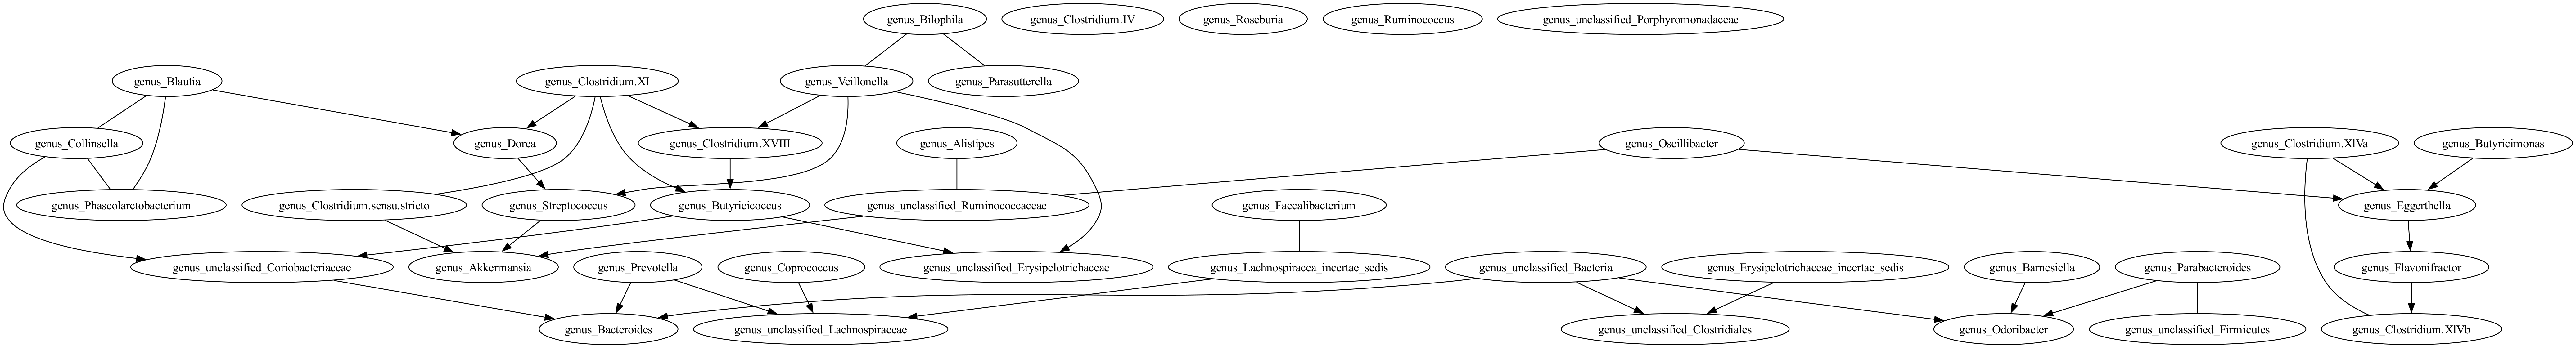
\includegraphics[width=\linewidth]{../graphs/t2d/glasso_IS_norm.png}
	\caption{Microbe-Microbe Network for T2D, IS cohort.}
    \end{figure}
    
    \begin{figure}
	
\includegraphics[width=\linewidth]{../graphs/t2d/glasso_IR_norm.png}
	\caption{Microbe-Microbe Network for T2D IR cohort.}
    \end{figure}
    
    \begin{itemize}
    	\item IR and IS cohorts share 21 microbes (Figures 2 and 3).
	\item IS have an additional three: \textit{Clostridium.XI, Clostridium.XIVa,} and \textit{Parasutterella}.
	\item IR have an additional four: \textit{Dorea, Ruminococcus, Veillonella,} and \textit{unclassified Ersipelotrichaceae}. 
    \end{itemize}
  \end{block}

\vspace{0.5cm}
% VAE Section
  \begin{block}{VAE}
    \begin{figure}[ht]
      \centering
      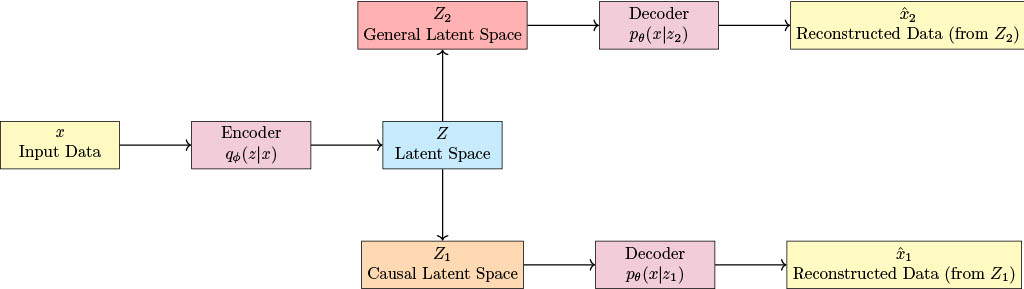
\includegraphics[width=\linewidth]{modified_vae.jpg} % Adjust the width as needed
      \caption{Baseline VAE}
      \label{fig:baseline_vae}
    \end{figure}

  \end{block}

  
\end{column}

\separatorcolumn

\begin{column}{\colwidth}

   \begin{block}{PCOS}

    % From the microbe-disease network (Figure 2), the following nine genera are causal to PCOS (`group' node): \textit{Alistipes, Blautia, Burkholderia, Desulfovibrio, Holdemanella, Knoellia, Prevotellaceae NK3B31 group, Ruminococcus,} and \textit{Ruminococcus gnavus group}. We find their individual causal effects with do-calculus (Table 2). 

    \begin{figure}
      \centering
      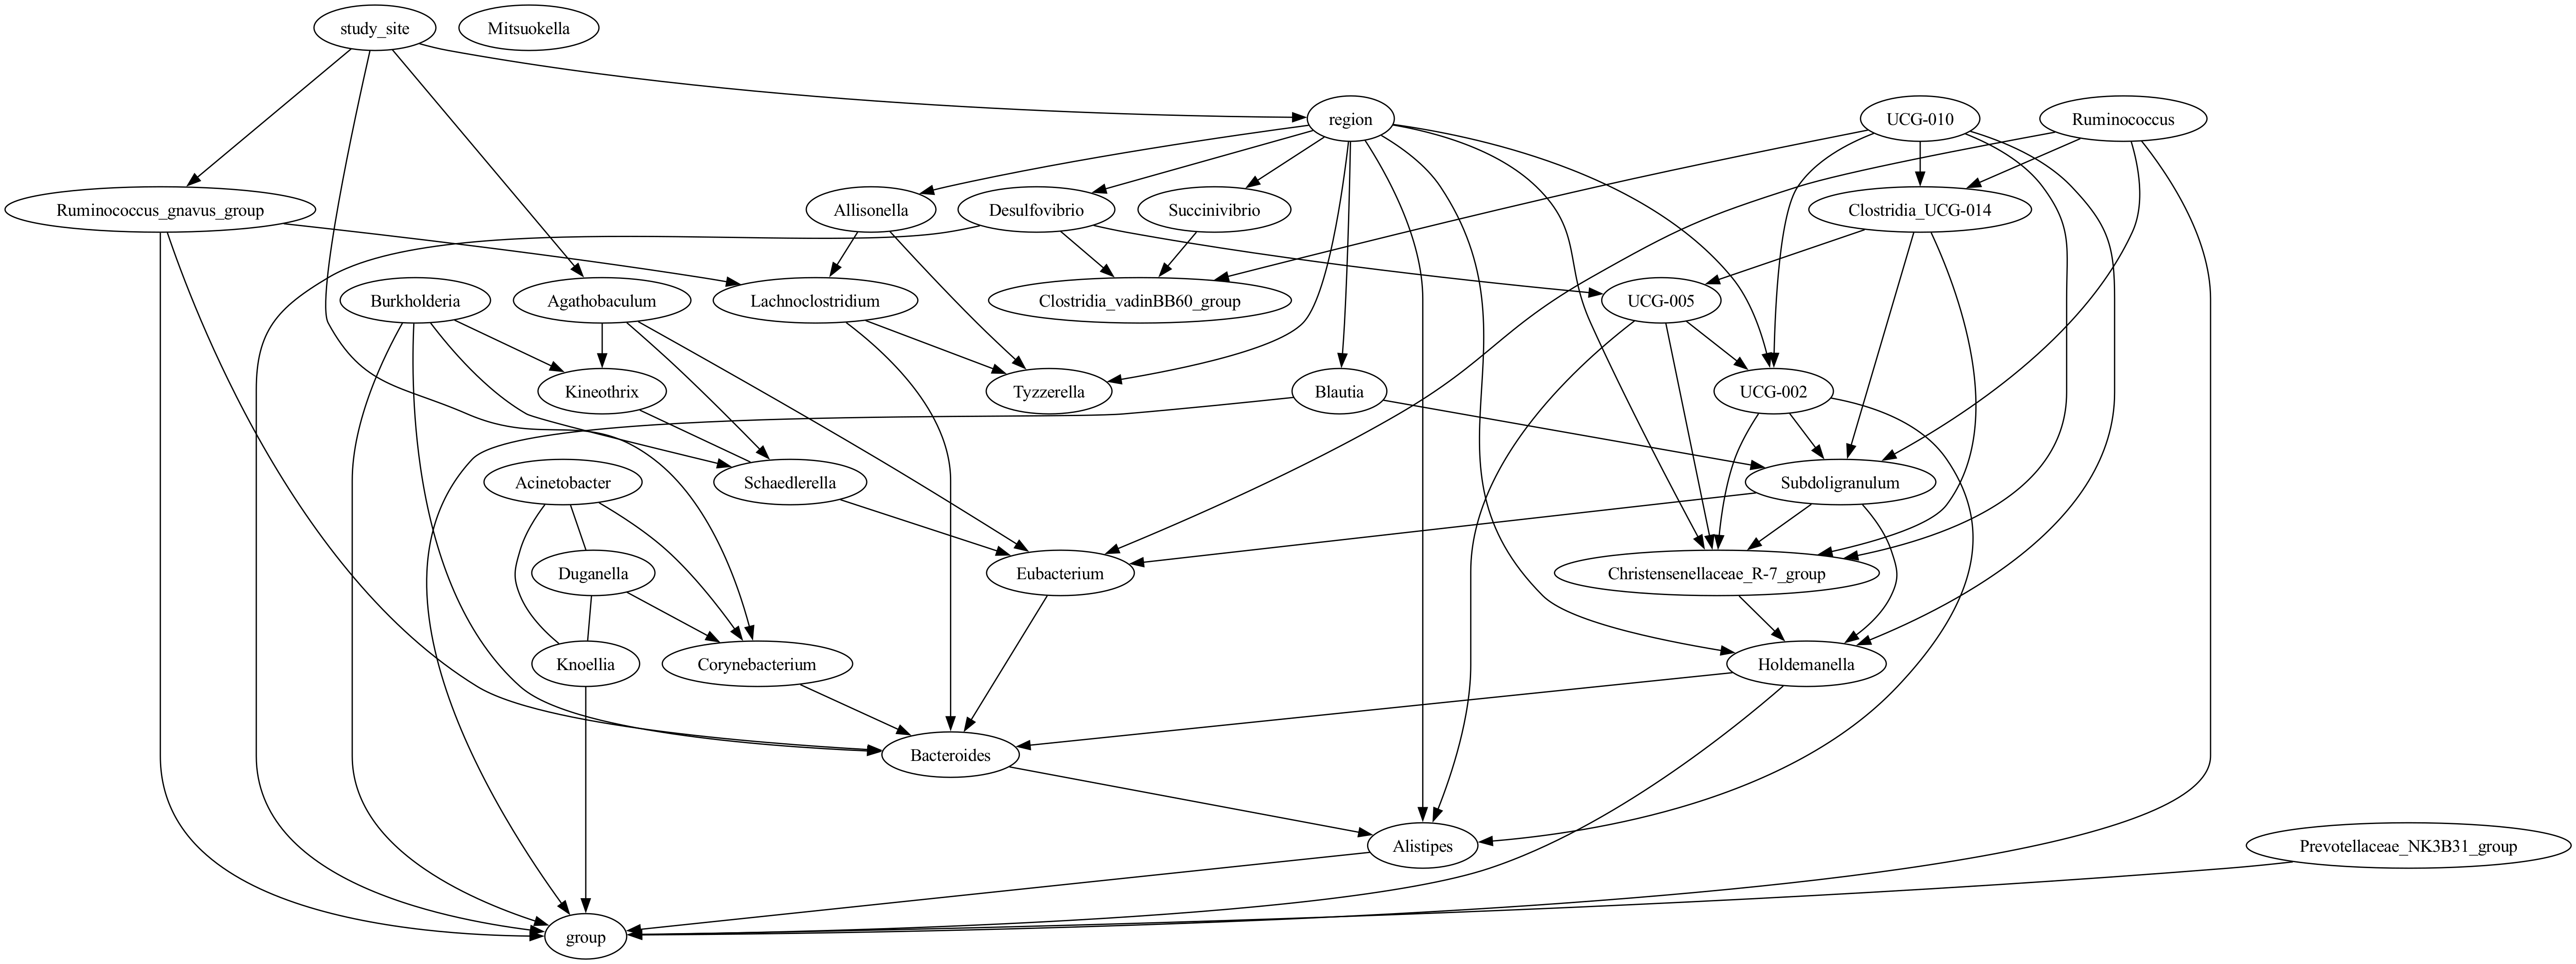
\includegraphics[width=\linewidth]{../graphs/pcos/cdnod_norm.png}
      \caption{Microbe-Disease Network for PCOS.}
    \end{figure}
    
    \begin{table}
      \centering
      \begin{tabular}{l r r r c}
        \toprule
        \textbf{Genus} & \textbf{Model 1} & \textbf{Model 2} & \textbf{BIRDMAn} & \textbf{Literature Agreement} \\
        \midrule
        \textit{Alistipes} & 0.13272* & 0.15346* & 1.28613* & Inconclusive \\
        \textit{Blautia} & 0.07461* & 0.07008* & 0.82554* & No \\
        \textit{Burkholderia} & -7.60599 & -0.48578 & -10.95696* & Inconclusive \\
        \textit{Desulfovibrio} & -0.79283* & -1.14492* & -0.17153 & No \\
        \textit{Holdemanella} & -0.22801* & -0.17267* & -0.13299 & Yes \\
        \textit{Knoellia} & 592.26751 & 1.40864 & 5.57650* & Inconclusive \\
        \textit{Prevotellaceae NK3B31 group} & -0.42407 & -0.47231* & -1.76743* & Inconclusive \\
        \textit{Ruminococcus} & -0.14137* & -0.13490* & -0.12796 & Inconclusive \\
        \textit{Ruminococcus gnavus group} & 0.24152* & 0.18259* & 2.01842 & Yes \\
        \bottomrule
      \end{tabular}
      \caption{Do-Calculus Results for PCOS.}
    \end{table}
    
    For the PCOS microbe-microbe networks, please see our website for the graphs and the specific differing microbes. \\
    \begin{itemize}
    	\item HC and PCOS cohorts share xx microbes.
	\item HC have an additional xxx. Includes (bring up a microbe-disease microbe). 
	\item PCOS have an additional xxx. Includes (bring up a microbe-disease microbe). 
    \end{itemize}

  \end{block}
  
  \vspace{0.5cm}

  \begin{block}{Conclusion \& Future Work}
  
  \begin{enumerate}
      \item \textbf{Microbe-Microbe:} Healthy and diseased participants share certain microbes, but also differ on which microbes are present and how they interact with other microbes. It is important to consider these microbes as communities of organisms rather than singular entities.      
      \item \textbf{Microbe-Disease:} Using CDNOD and do-calculus, we are able to quantify the effects of microbes on disease status, and they agree with microbiome-specific differential analysis methods such as BIRDMAn, and they also mostly agree with current literature.
      \item \textbf{Prediction:} We find that baseline models like logistic regression perform better than the VAE model. Due to the complexity of the model, we may require more hyper parameter tuning or longitudinal data for the VAE to be on par with baseline models.
   \end{enumerate}
   
   Our work can be improved to adjust for multiple testing and low statistical power, use different causal discovery algorithms for different data structures (e.g. longitudinal, meta-analyses, etc.) and account for compositionality and rareness in gut microbiome data. 
	
	\begin{wrapfigure}{r}{0.2\textwidth}
           \centering
           
\includegraphics[width=\linewidth]{website_qr.png}
    	\end{wrapfigure} We hope this project shows the potential of causal discovery and causal inference methods in human gut microbiome research, and can be generically applied to other diseases of interest. We would like to thank our mentors, Dr. Biwei Huang \& Dr. Jelena Bradic,  and Dr. Sam Degregori (Knight Lab) for guidance throughout this project.
    
  \end{block}

%    \begin{block}{References}
%    
%    \footnotesize{\bibliographystyle{unsrt}\bibliography{../report/reference}}
%    
%    \end{block}

\end{column}

\separatorcolumn
\end{columns}
\end{frame}

\end{document}